% Source: graduate-coursework/Prior_Semesters/Fa25/EMCH501/HW2/HW2.tex

\documentclass[border=4pt]{standalone}
\usepackage{amsmath}
\usepackage{amssymb}
\usepackage{graphicx}
\usepackage{tikz}
\usepackage{xcolor}
\usetikzlibrary{shapes.geometric, arrows.meta, positioning, decorations.pathmorphing, patterns}

\begin{document}
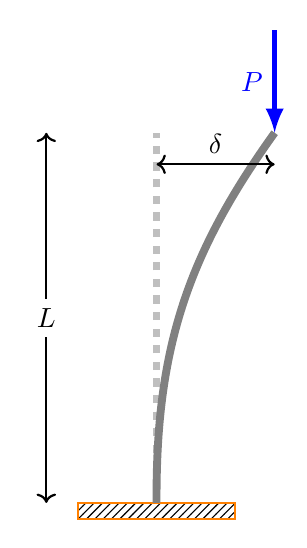
\begin{tikzpicture}[scale=1.0]
  % ground support
  \draw[pattern=north east lines, draw=orange, thick] (-1,0) rectangle (1,-0.2);
  % original column (dashed)
  \draw[line width=1mm, dashed, lightgray] (0,0) -- (0,4.7);
  % deflected shape
  \draw[line width=1mm, gray] (0,0) to[bend left=18] (1.5,4.7);
  % length dimension
  \draw[<->, thick] (-1.4,0) -- node[midway,fill=white] {$L$} (-1.4,4.7);
  % tip displacement
  \draw[<->, thick] (0,4.3) -- node[above] {$\delta$} (1.5,4.3);
  % applied load
  \draw[-latex, line width=.7mm, blue] (1.5,6) -- node[left] {$P$} (1.5,4.7);
\end{tikzpicture}
\end{document}
